\section{On the number of types in sparse graph classes}\label{sec:types}

In this section we prove \Cref{thm:vc-density} and \Cref{thm:vc-density-lower-bound}.
	Recall that \Cref{thm:vc-density} provides upper bounds on the number of types in classes of graphs which are nowhere dense, 
	and stronger bounds for classes which have bounded expansion. 
	On the other hand, the complementary \Cref{thm:vc-density-lower-bound} shows that for subgraph-closed classes, in the absence of structural sparsity we cannot hope for such upper bounds.

\paragraph*{Upper bounds for sparse classes.}
We first concentrate on proving \Cref{thm:vc-density}.
From now on we fix a formula  $\phi(\tup x,\tup y)$ where
$\tup x$ is an $m$-tuple and $\tup y$ is an $n$-tuple of variables.

% For a graph $G$, a set of  vertices $A\subset V(G)$, and a tuple $\tup v\in V(G)^n$,
% denote
% \[\phi(A,\tup v)=\setof{\tup a \in A^m }{ G\models\phi(\tup a,\tup v)}.\]
% We call $\phi(A,\tup v)$ the \emph{$\phi$-type} of $\tup v$ \emph{over} $A$, and
% $A$ is sometimes called the \emph{parameter set}.
% For $W\subset V(G)$, denote
% \[S_\phi(A,W)=\setof{\tp^\phi_G(\bar v/A)}{ \tup v\in W^n}.\]
% Note that $S_\phi(A,W)$ is \emph{not} symmetric in $A$ and $W$.
% We write $S_\phi(A,G)$ as a shorthand for $S_\phi(A,V(G))$.
% The set $S_\phi(A,G)$ is therefore the set of all $\phi$-types of $n$-tuples
% of vertices of $G$ over the parameter set $A$.
Our goal is to prove that if $G\in \CCC$, where $\CCC$ is a nowhere dense class,
then for every $\varepsilon>0$ we have  $|S^\phi(G/A)|\le \Oof(|A|^{n+\varepsilon})$, and 
if $\CCC$ is moreover of bounded expansion, then in fact $|S^\phi(G/A)|\le \Oof(|A|^n)$.


To prove~\cref{thm:vc-density},
we will first enlarge the set $A$ to a set $B$, called
an \emph{$r$-closure of $A$}, such 
that the connections of elements from $V(G)\setminus B$ 
towards $B$ are well controlled. This approach
was first used in Drange et al.~\cite{drange2016kernelization} in the context of classes of bounded expansion, 
and then for nowhere dense classes in Eickmeyer et al.~\cite{eickmeyer2016neighborhood}. 
Let us recall the necessary definitions.

Let $G$ be a graph and let $B\subseteq V(G)$ be a subset of vertices. For vertices $v\in B$ and $u\in V(G)$, a path $P$ connecting $u$ and $v$ is called {\em{$B$-avoiding}}
if all its vertices apart from~$v$ do not belong to $B$. For a positive integer $r$ and $u\in V(G)$, the {\em{$r$-projection}} of $u$ on $B$, denoted $M^G_r(u,B)$, is the set of all vertices $v\in B$ that
can be connected to $u$ by a $B$-avoiding path of length at most $r$. Note that for $u\in B$, we have $M^G_r(u,B)=\{b\}$.
Equivalently, $M^G_r(u,B)$ is the inclusion-minimal
subset of $B$ which $r$-separates $u$ from $B$.

%
%The {\em{$r$-projection profile}} of a vertex $u\in V(G)\setminus A$ on $A$ is a function $\rho^G_r[u,A]$ mapping vertices of
%$A$ to $\{0,1,\ldots,r,\infty\}$, defined as follows: for every $v\in A$, the value $\rho^G_r[u,A](v)$ is the length of a shortest $A$-avoiding path connecting $u$ and~$v$, and~$\infty$ in case this length
%is larger than $r$. 
%
\begin{comment}
\begin{figure}[h!]
	\centering
		\includegraphics[scale=0.35,page=2]{pics}
	\caption{The  $r$-projection of $u$ on $B$
	(here $r=2$)
	is the minimal (inclusion-wise) set of $S\subset B$
	which $r$-separates $ u$ from $B$.
	}
	\label{fig:gaifman}
\end{figure}
\end{comment}

We define 
\[\projnum_r(G,B)=|\{M_r^G(u,B)\colon u\in V(G)\}|\]
%\quad\textrm{and}\quad \projprof_r(G,A)=|\{\rho_r^G[u,A]\colon %u\in V(G)\setminus A\}|\]
to be the number of different $r$-projections on $B$.
In the sequel, we will need the following results from~\cite{drange2016kernelization,eickmeyer2016neighborhood}.
% and $r$-projection profiles realized on $B$, respectively. Clearly, it %holds that $\projnum_r(G,A)\leq \projprof_r(G,A)$.

\begin{lemma}[\cite{drange2016kernelization}]\label{lem:closure-be}
Let $\CCC$ be a class of bounded expansion. 
Then for every $r\in \N$ there is a constant $c\in \N$ such that for
every $G\in \CCC$ and $X\subseteq V(G)$ there exists a set $\cl_r(X)$, called an {\em{$r$-closure}} of $X$, with the following properties. 
\begin{enumerate}[(a)]
  \item $X\subseteq \cl_r(X)\subseteq V(G)$;
  \item $|\cl_r(X)|\leq c\cdot |X|$; and
  \item $|M_r^G(u,\cl_r(X))|\leq c$ for each $u\in V(G)$.
\end{enumerate}
\end{lemma}

\begin{lemma}[\cite{eickmeyer2016neighborhood}]\label{lem:closure-nd}
Let $\CCC$ be a nowhere dense class. 
Then for every $r\in\N$ and $\epsilon>0$ there is a 
constant $c\in\N$ such that for every $G\in \CCC$ and $X\subseteq V(G)$ there exists a set 
$\cl_r(X)$,  called an {\em{$r$-closure}} of $X$, 
with the following properties: 
\begin{enumerate}[(a)]
  \item $X\subseteq \cl_r(X)\subseteq V(G)$;
  \item $|\cl_r(X)|\leq c\cdot |X|^{1+\epsilon}$; and
  \item $|M_r^G(u,\cl_r(X))|\leq c\cdot |X|^{\epsilon}$ for each $u\in V(G)$.
\end{enumerate}
\end{lemma}

\begin{lemma}[\cite{drange2016kernelization}]\label{lem:projection-complexity-be}
Let $\CCC$ be a class of bounded expansion. Then for every $r\in \N$ there is 
  a constant $c\in\N$ such that for every graph $G\in \CCC$ and vertex subset $A\subseteq V(G)$, 
  it holds that $\projnum_r(G,A)\leq c\cdot |A|$.
\end{lemma}

\begin{lemma}[\cite{eickmeyer2016neighborhood}]\label{lem:projection-complexity-nd}
Let $\CCC$ be a nowhere dense class. Then for every $r\in \N$ and $\epsilon>0$ there is 
  a constant $c\in \N$ such that for every graph $G\in \CCC$ and vertex subset $A\subseteq V(G)$, 
  it holds that $\projnum_r(G,A)\leq c\cdot |A|^{1+\epsilon}$.
\end{lemma}

We note that in~\cite{drange2016kernelization,eickmeyer2016neighborhood} projections on $B$ are defined only for vertices outside of $B$. 
However, adding singleton projections for vertices of $B$ to the definition only adds $|B|$ possible projections of size $1$ each, so this does not influence the validity of the above results.

\begin{comment}
\begin{figure}[t]
	\centering
		\includegraphics[scale=0.35,page=3]{pics}
	\caption{Summarization of closures and projections in the nowhere dense case, i.e., \Cref{lem:closure-nd} and \Cref{lem:projection-complexity-nd}. The $r$-closure $B$ of $A$ has the following three properties:
(a) its size is  $\Oof(|A|^{1+\epsilon})$,
(b) it has at most $\Oof(|B|^{1+\epsilon})$ distinct $r$-projections,
(c) every $r$-projection has size $\Oof(|B|^\epsilon)$.
}
	\label{fig:closure}
\end{figure}

We informally sketch our proof of~\cref{thm:vc-density} in Figure~\ref{fig:sketch}.
\begin{figure}[h!]
	\centering
		\includegraphics[scale=0.35,page=4]{pics}
	\caption{Sketch of the proof of~\cref{thm:vc-density}. The precise values $\epsilon_1,\ldots,\epsilon_5$ need to be adapted suitably.
	%We rescale $\epsilon$	freely in the arguments.
	Fix $\phi$ of quantifier rank $q$ and let 
$r$ be the number obtained from~\cref{pro:crossing}.
Let $B$ be the $r$-closure of $A$. 
	Suppose that there are $|B|^{1+\epsilon_1}$ nodes with
	mutually distinct $\phi$-types over $B$.
	In the first step, we extract a set of $|B|^{\epsilon_3}$
	nodes which have the same $r$-projection $C$ to $B$;
	thus, they are $r$-separated from $B$ by $C$.
In the second step, using uniform quasi-wideness
with polynomial bounds,
	we further extract a subset of $|B|^{\epsilon_3/d}=|B|^{\epsilon_4}$ nodes
	(where $d$ is some constant)
	 which 
	are pairwise $2r$-separated by $S$, for some set of vertices $S$
	of constant size.
Since $|C|\le|B|^{\epsilon_2}$ 
it is easy to see that among these
	$|B|^{\epsilon_4}$ nodes,
there must be $|B|^{\epsilon_5}$
nodes which are $r$-separated from $B$ by $S$.
	Since $|S|$ is a constant,
	there is only a constant number of $(q,S)$-local types,
	so there must be two nodes $u,v$
	with the same $(q,S)$-local types, 
	which are $r$-separated from $B$ by $S$.
	By~\cref{pro:crossing}, $u$ and $v$ have the same types over $B$. This is a contradiction with the assumption the initial nodes $|B|^{1+\epsilon_1}$ had distinct $\phi$-types over $B$.	
	}
	\label{fig:sketch}
\end{figure}
For a formal proof, we formulate the following lemma,
which corresponds to the reasoning depicted in the figures caption,
starting from the point where a set of vertices with the same $r$-projection has been already selected.
\end{comment}

\Cref{thm:vc-density} will follow easily from the above results and the following lemma.

\begin{lemma}\label{lem:num-types-same-class}
Let $\CCC$ be a nowhere dense class.
Then there exists a polynomial $p(\cdot)$, depending only on $\CCC$ and the fixed formula $\phi$, such that for every graph $G\in\CCC$ and all sets of its vertices $B,C$ with
$C\subset B\subseteq V(G)$, the following holds.
For every set of vertices $W\subseteq V(G)$ such that 
$M_r^G(u,B)\subseteq C$ for all $u\in W$, 
we have $|S^\phi(W/B)|\le p(|C|)$.
\end{lemma}
\begin{proof}
Let $q$ be the quantifier rank of the formula $\phi$.
Let $p,r\in \N$ be as in~\cref{lem:types}.
% ~$T\from \N\times \N\times \N\to \N$
% be as described in~\cref{pro:crossing} for the quantifier rank $q$.

Let $N^d\colon \N\times\N\to\N$ and $s^d\colon \N\to\N$ be
the functions for $\CCC$ described in \Cref{prop:uqw-tuples}. 
Let $s=s^n(2r)$, that is, we apply the function $s^d(\cdot)$ to
parameters $d=n$ and $2r$, and let $k\coloneqq T(q,d,s)$,
where $T$ is the function from~\cref{lem:types}.
That is, $k$ is an upper bound on the number 
of quantifier-rank $p$ types of $d$-tuples of vertices, with parameters from a set of size $s$.
Note that  $k$ is computable from $q,d$ and $s$.
% As noted
% $\coloneqq T(q,n,s)$. In the parlance of~\cref{pro:crossing},
% $k$ is an upper bound on the number of $(q,S)$-local types of vertices in any graph~$G$,
% for any fixed $S\subset V(G)$ with $|S|\le s$.
 Recall that according
to \Cref{prop:uqw-tuples}, the function $N^d(\cdot,\cdot)$ is polynomial in the second
argument. 

Let $Y\subseteq W^n$ be a maximal set of $n$-tuples 
such that $\phi(B,\tup u)\neq \phi(B,\tup v)$ 
for any distinct $\tup u, \tup v\in Y$.
Suppose $|Y|\geq N^n(r,k+c+1)$. Then, by \Cref{prop:uqw-tuples}, there is a  
set $S\subseteq V(G)$ of size $|S|\leq s$ 
and a set $X\subseteq Y$ of size $|X|\geq k+c+1$ which is 
mutually $2r$-independent in $G-S$. 
%\textcolor{red}{Furthermore, 
%on each coordinate that contains an element of $S$ we have 
%equality for all tuples. We now need a lemma that this is fine.} 

Consider function $\pi\from V(G)\to 2^C$
defined as
 $\pi(v)\coloneqq M_r^{G-S}(v,B)$; note that $\pi(v)=\emptyset$ whenever $v\in S$.
 Then, for distinct $\tup v,\tup w\in X$
 and $1\leq i,j\leq n$, if by $v_i$ and $w_j$ we denote the $i$th and the $j$th coordinate of $\tup v$ and $\tup w$, respectively, then 
 the sets $\pi(v_i)$ and $\pi(w_j)$ are pairwise disjoint subsets of $C$,
as otherwise we would have \mbox{$\dist_{G-S}(v_i,w_j)\leq 2r$},
contradicting mutual $2r$-independence.
As  $|X|\ge k+|C|+1$, it follows that 
there are at least $k+1$ tuples $\tup v\in X$
such that  $\pi(v)=\emptyset$ for every vertex $v$ appearing in $\bar v$. Let $Z\subseteq X$ denote the set of these tuples. Since
$M_r^G(u,B)\subseteq C$ for all $u\in W$, it follows that the set of all vertices appearing in~$Z$ and the
set $B$ are $r$-separated by~$S$.

Since $|Z|\geq k+1$, there are  distinct $\tup v,\tup w\in Z$ such that 
$\tup v$ and $\tup w$ have the same quantifier rank $q$ type over $S$.
From~\cref{lem:types} it follows that $\tup v$ and $\tup w$
have the same quantifier rank $q$ type over~$B$,
i.e., $\tp^q(\bar v/B)=\tp^q(\bar w/B)$. Since $\tup v,\tup w\in Y$, this contradicts the definition of $Y$. 
This proves $|Y|<N^n(r,k+c+1)$, hence $|S^\phi(W/B)|=|Y|<p(c)$ for $p(c)= N^n(r,k+c+1)$.
\end{proof}

We now use all the above tools to prove \Cref{thm:vc-density}. We repeat its statement for convenience.

\setcounter{theorem}{2}
\begin{theorem}
Let $\CCC$ be a class of graphs and let $\psi(\tup x,\tup y)$ be a first-order formula, where 
$\tup x$ is an $m$-tuple and $\tup y$ is an $n$-tuple of variables. 
\begin{enumerate}[(1)]
\item If $\CCC$ is nowhere dense, then for every $\epsilon>0$ 
there exists a constant~$c$ such that for every $G\in \CCC$ and every nonempty
$A\subseteq V(G)$, we have $|S^\psi(G/A)|\leq c\cdot |A|^{n+\epsilon}.$

\item If $\CCC$ has bounded expansion, then there exists a constant~$c$ such that for every $G\in \CCC$ and every nonempty $A\subseteq V(G)$, we have $|S^\psi(G/A)|\leq c\cdot |A|^n$.
\end{enumerate}
\end{theorem}

\begin{proof}
We prove the statement about nowhere dense classes of graphs,
the bounded expansion case is proved analogously using \Cref{lem:closure-be} and \Cref{lem:projection-complexity-be} instead of \Cref{lem:closure-nd} and \Cref{lem:projection-complexity-nd}.

Let $p(\cdot)$ be the polynomial provided by \Cref{lem:num-types-same-class},
depending on $\phi$ and $\CCC$. Assume $p(x)\leq c_0x^d$ 
for some constants $c_0$ and $d$. 
Choose $\epsilon'>0$ so that $(2n+d)\epsilon'+n\epsilon'^2=\epsilon$. 

Let $B$ be an $r$-closure of $A$ according to \Cref{lem:closure-nd} for parameter $\epsilon'$. 
According to the lemma, 
there is a constant $c_1$ such that 
we have $|M_r^G(u,B)|\leq c_1\cdot |A|^{\epsilon'}$ 
for each $u\in V(G)$ and 
$|B|\leq c_1\cdot |A|^{1+\epsilon'}$. According to 
\Cref{lem:projection-complexity-nd}, applied
with parameters $r$ and $\epsilon'$, 
there is a constant
$c_2$ such that 
$$\projnum_r(G,B)\leq c_2\cdot |B|^{1+\epsilon'}\leq
c_2\cdot (c_1\cdot |A|^{1+\epsilon'})^{1+\epsilon'}=c_1^{1+\epsilon'}c_2\cdot|A|^{1+2\epsilon'+\epsilon'^2}.$$
As $A\subseteq B$, 
according to \Cref{lem:types-over-B} it suffices to bound the
number $|S^\phi(G/B)|$. 

We define an equivalence relation $\sim_r$ on 
$V(G)$ by $u\sim_r v$ iff 
$M_r^G(u,B)=M_r^G(v,B)$. 
Fix any $n$ equivalence
classes $\kappa_1,\ldots, \kappa_n$ (not necessarily
distinct) of $\sim_r$. Let $C=\bigcup_{1\leq i\leq n}M_r^G(u_i, B)$, 
where $u_i\in \kappa_i$ is any representative of the
equivalence class $\kappa_i$. Observe that $C\subseteq B$ with
$|C|\leq n\cdot c_1\cdot |A|^{\epsilon'}$. 
Then, according to \Cref{lem:num-types-same-class}, 
we have $|S^\phi(\bigcup_{1\leq i\leq n}\kappa_i/B)|\leq
c_0\cdot |C|^d$. 

As we have at most $\mu_r(G,B)^n$ choices for 
$\kappa_1,\ldots, \kappa_n$, we may bound the total 
number of types as follows:
\begin{align*}
|S^\phi(G/A)| & \leq |S^\phi(G/B)|\leq \mu_r(G,B)^n \cdot c_0\cdot |C|^d\\
& \leq \left(c_1^{1+\epsilon'}c_2|A|^{1+2\epsilon'+\epsilon'^2}\right)^n\cdot c_0\left(nc_1|A|^{\epsilon'}\right)^d\\
& = c_0c_1^{(1+\epsilon')n+d}c_2^nn^d|A|^{n+(2n+d)\epsilon'+n\epsilon'^2} = c_0c_1^{(1+\epsilon')n+d}c_2^nn^d|A|^{n+\epsilon}.
\end{align*}
Hence, taking $c\coloneqq c_0c_1^{(1+\epsilon')n+d}c_2^nn^d$ finishes the proof.
\end{proof}

\paragraph*{Lower bounds for non-sparse classes.}
We now move to the proof of \Cref{thm:vc-density-lower-bound}, which we also repeat for
convenience.

\begin{theorem}
Let $\CCC$ be a class of graphs which 
is closed under taking subgraphs. 
\begin{enumerate}[(1)]
\item If $\CCC$ is somewhere dense, then there is a formula 
$\psi(x,y)$ such that for every $n\in \N$ there are $G\in\CCC$ and $A\subseteq V(G)$ 
with $|A|=n$ and $S^\psi(G/A)=2^{A}$. 
\item If $\CCC$ has unbounded expansion, then there is a formula 
$\psi(x,y)$ such that for every $c\in \mathbb{R}$ there exist $G\in\CCC$ and $A\subseteq V(G)$ with $|S^\psi(G/A)|>c|A|$. 
\end{enumerate}
\end{theorem}

\Cref{thm:vc-density-lower-bound} is a simple consequence of the following two
known results. 
Let $\mathcal{G}_r$ be the class of $r$-subdivisions of all 
simple graphs, that is, the class comprising
all the graphs that can be obtained from any simple graph by replacing every edge by a path of
length $r$.

\begin{lemma}[\cite{nevsetvril2011nowhere}]\label{lem:lower-nd}
For every somewhere dense graph class $\CCC$ that is closed 
under taking subgraphs, there
exists an integer $r_0$ such that $\mathcal{G}_{r_0}\subseteq \CCC$.
\end{lemma}

A graph $H$ is a \emph{topological depth-$r$ minor} of $G$ if
there is a mapping $\phi$ that maps vertices of~$H$ to 
vertices of $G$ such that $\phi(u)\neq \phi(v)$ for 
$u\neq v$, and edges of $H$ to paths in 
$G$ such that if $uv\in E(H)$, then $\phi(uv)$
is a path of length at most $2r$ between $u$ and $v$ in 
$G$ and furthermore, if $uv, xy\in E(H)$, then 
$\phi(uv)$ and $\phi(xy)$ are internally vertex
disjoint. We write $H\minor_r^t G$. 
Note that the above definition makes sense for 
half-integers, i.e., numbers $r$ for which $2r$ is an integer.

Dvov{r}\'ak proved that classes of bounded expansion can be alternatively characterized by the sparsity of shallow topological minors.

\begin{lemma}[Theorem {\bf{TODO}} of \cite{dvorak2007asymptotical}]\label{lem:top-bnd-exp}
A class $\CCC$ of graphs has bounded expansion if and only 
if for every $r\in \N$ there exists a constant $c_r$ such that $|E(H)|/|V(H)|\leq c_r$ for all graphs $H$ such that $H\minor_r^tG $ for some $G\in \CCC$.
\end{lemma}

For $r\in \N$ and a graph $G$ denote by $\nu_r(G)$ the
\emph{$r$-neighborhood complexity} of $G$ as defined
by Reidl et al.~\cite{reidl2016characterising}, that is, the number 
\[\max_{H\subseteq G,\,\emptyset\neq X\subseteq V(G)}\frac{|\{N_r^H[v]\cap X : v\in V(H)\}|}{|X|}.\] 
We will need the following result relating edge density in shallow topological minors and neighborhood complexity.

\begin{lemma}[Theorem 4 of \cite{reidl2016characterising}]\label{lem:lower-be}
Let $G$ be a graph, $r$ be a half-integer, 
and let $H\minor_r^tG$. 
Then 
$$\frac{|E(H)|}{|V(H)|}\leq (2r + 1)\cdot \max \left\{\nu_1(G)^4\cdot \log^2\nu_1(G),\nu_2(G),\ldots, \nu_{\left\lceil r+\frac{1}{2}\right\rceil}(G)\right\}.$$
\end{lemma}

With the known results stated, we proceed to the proof of \Cref{thm:vc-density-lower-bound}.

\begin{proof}[of \Cref{thm:vc-density-lower-bound}]
To prove the first statement of \Cref{thm:vc-density-lower-bound}, 
for $n\in \N$, let $P(n)$ denote the graph with $n+2^n$ 
vertices $V(P(n))\coloneqq \{v_1,\ldots, v_n\}\cup \{w_M \colon M\subseteq \{1,\ldots, n\}\}$ and edges $E(P(n))\coloneqq \{v_iw_M \colon 1\leq i\leq n,\, M\subseteq \{1,\ldots, n\},\, i\in M\}$. 
If $\CCC$ is somewhere dense and closed under taking subgraphs, 
according to \Cref{lem:lower-nd}, there exists an integer $r_0$ 
such that $\mathcal{G}_{r_0}\subseteq \CCC$. In particular, for every $n\in \N$ the $r_0$-subdivision of graph $P(n)$ is contained in $\CCC$.
Now consider 
the formula $\psi(x,y)$ stating that $x$ and~$y$ are at distance at most $r_0$. Then for every $n\in \N$ we have 
$S^\psi(P(n)/A)=2^{|A|}$, where $A\subseteq V(P(n))$ denotes the set $\{v_1,\ldots, v_n\}$. This implies the first statement
of the theorem.

For the second claim, we use the contrapositive of \Cref{lem:top-bnd-exp}: since $\CCC$ has unbounded expansion, for some $r\in \N$ 
we have that the value $|E(H)|/|V(H)|$ is unbounded among depth-$r$ topological minors $H$ of graphs from $\CCC$.
By applying \Cref{lem:lower-be}, we find that for some $r_0\leq r$, the value
$\nu_{r_0}(G)$ is unbounded when $G$ ranges over all graphs from $\CCC$. 
As above, consider the formula $\psi(x,y)$ stating that $x$ and~$y$ are at distance at most $r_0$ to conclude. 
\end{proof}

